\section{Fonctionnalités implémentées}
\subsection{Type de voisinage}
Nous avons développé la fonctionnalité \textbf{type de voisinage}. Cette fonctionnalité consiste à
déterminer quels sont les voisins d’une cellule. Par défaut dans le jeu de la vie, ces voisins
sont les huit voisins directs de la cellule. Nous avons fait en sorte que les voisins puissent
être configurables. Un voisin pourrait être par exemple \textbf{la deuxième cellule à droite ou
encore la troisième cellule à gauche de deux lignes au-dessus}. Étant donné une cellule
de coordonnées \textbf{(x,y)}, ces voisins correspondraient donc respectivement aux cellules de
coordonnées \textbf{(x,y+2) et (x-2,y-3)}. Pour implémenter cela, nous avons attribué à notre
\textbf{générateur} un tableau des voisins d’une cellule correspondant aux positions de ces voisins
relativement à la cellule comme décrit précédemment. Ainsi, pour compter le nombre de
voisins vivants d’une cellule, nous n’avons qu’à parcourir ce tableau, récupérer les cellules
aux positions correspondantes et incrémenter un compteur à chaque fois qu’on tombe sur une cellule vivante.
\subsection{Type de règles}
Nous avons implémenté une fonctionnalité qui permet à l'utilisateur de choisir la règle qu'il souhaite utiliser. Contrairement à la règle classique du jeu de la vie qui impose l'utilisation de la règle \textbf{B3/S23}, notre programme permet \textbf{à l'utilisateur de spécifier sa propre règle}. Pour ce faire, nous avons créé une interface appelée \textbf{"RuleFormat"} qui regroupe deux méthodes : \textbf{read et check}. La méthode read permet de lire une règle tandis que la méthode check permet d'appliquer cette règle en fonction du nombre de voisins.

Nous avons également créé deux classes qui implémentent l'interface RuleFormat. La première classe, nommée \textbf{"RuleMulttF"}, permet d'implémenter une règle au format \textbf{"xy"} tandis que la seconde classe, nommée \textbf{"RuleRangeF"}, permet d'implémenter une règle de type \textbf{"x-y"}. Nous avons ensuite utilisé une classe appelée \textbf{"Rule"} pour traiter une règle spécifique. Cette classe contient une méthode "read" qui permet de lire une règle entrée par l'utilisateur et d'instancier soit la classe RuleMulttF soit la classe RuleRangeF en fonction de la forme de la règle.

Par exemple, si l'utilisateur entre la règle \textbf{"B23/S2-3"}, l'attribut \textbf{"bornRule"} de la classe Rule sera initialisé en instanciant la classe RuleMulttF tandis que l'attribut \textbf{"surviveRule"} sera initialisé en instanciant la classe RuleRangeF. De plus, nous avons ajouté une méthode "checkBorn" qui appelle la méthode "check" sur l'attribut "bornRule" et une méthode "checkSurvive" qui appelle la méthode "check" sur l'attribut "surviveRule".Il est à noter que nous avons utilisé des expressions régulières (regex) pour vérifier la validité de la règle entrée par l'utilisateur. Cette organisation permet une meilleure structure et efficacité de notre programme
\subsection{Patterns}
Nous avons ajouté une fonctionnalité pour que les joueurs puissent commencer une partie avec une \textbf{grille personnalisée}. Pour cela, nous avons implémenté la méthode "initPattern" qui permet d'initialiser la grille de jeu en se basant sur les informations contenues dans un fichier texte. Cette méthode prend en paramètre le nom du fichier à lire.

La première étape de la méthode consiste à \textbf{créer une matrice appelée "pattern"} qui aura la même taille que la grille de jeu, définie par les attributs "nbLine" et "nbColumn" de l'objet.

Ensuite, la méthode utilise un objet "Scanner" pour ouvrir le fichier texte et parcourir chaque ligne. Pour chaque ligne lue, la méthode examine chaque caractère et vérifie s'il s'agit d'un 0, d'un 1 ou d'un caractère invalide. Si le caractère est valide, il est stocké dans la matrice "pattern" à l'indice correspondant.

La méthode vérifie également que le nombre de lignes et de colonnes lues ne dépasse pas le nombre de lignes et de colonnes de la grille de jeu. Si cette condition n'est pas remplie, une exception est levée.

Une fois que toutes les lignes ont été lues et que la matrice "pattern" est remplie, la méthode calcule les indices de départ pour placer la matrice "pattern" dans la grille de jeu. Ces indices sont calculés pour centrer la matrice "pattern" dans la grille.

Enfin, la méthode parcourt la matrice "pattern" et place chaque élément dans la grille de jeu à l'indice correspondant. Si une exception est levée pendant la lecture du fichier, un message d'erreur s'affiche sur la console
\begin{figure}[h]
		\centering
      \raggedright  
		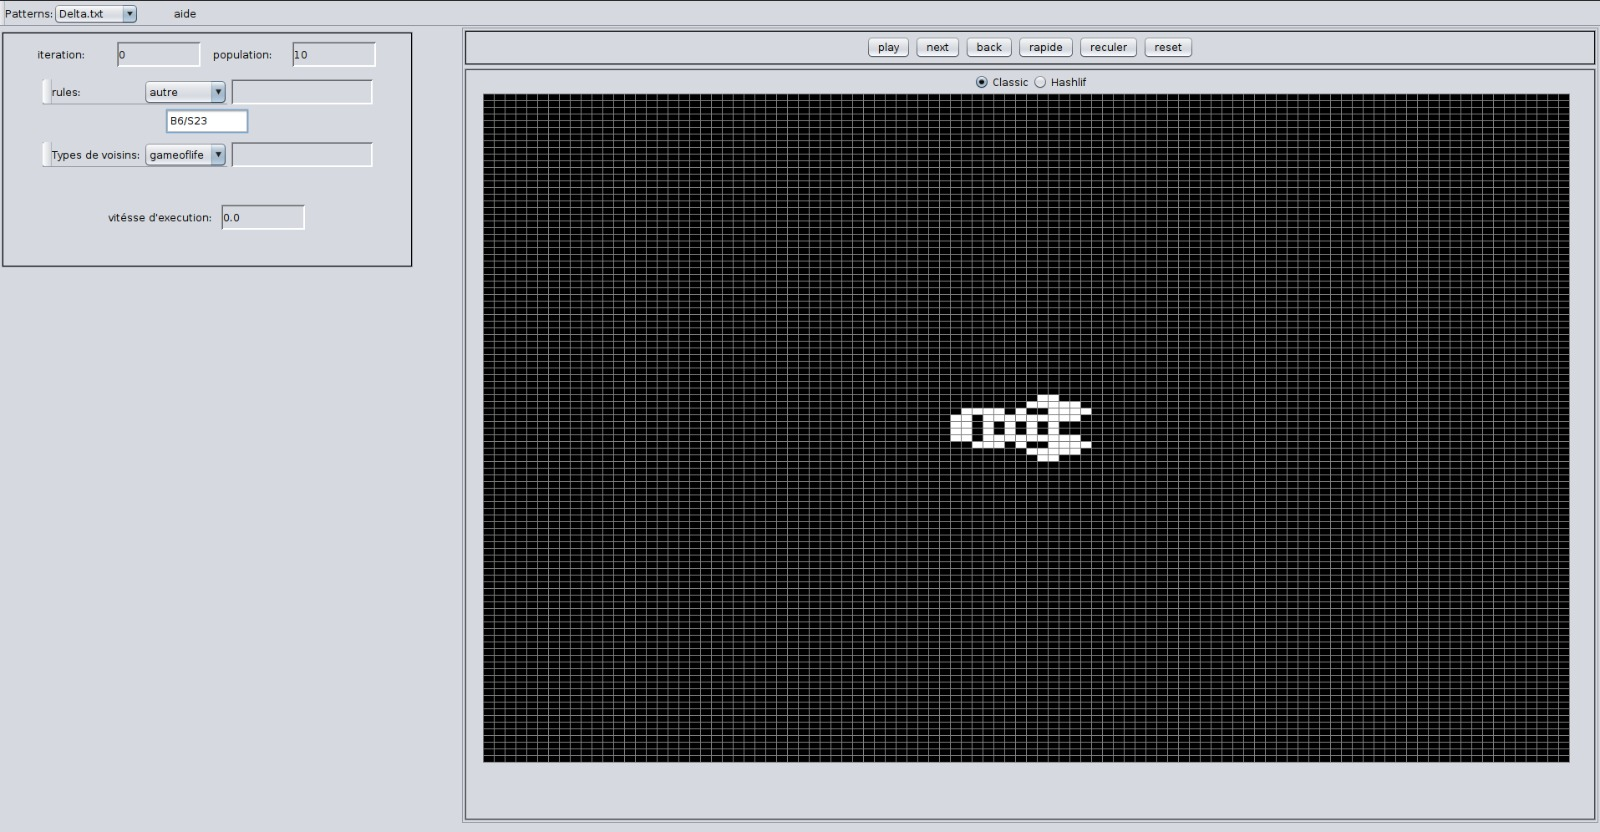
\includegraphics[width=13cm]{images/image1.jpeg}
	    \caption{exemple de la grille inialisée avec un pattern }
\end{figure}
\newpage
\subsection{Hashlife}
\subsubsection{Hashlife de quoi s'agit t'il ?}

HashLife est un algorithme qui améliore considérablement l'efficacité du calcul en \textbf{permettant de sauter plusieurs générations et d'évoluer rapidement une grille sur des milliers voire des millions de générations en une seule étape}. En outre, il utilise une représentation mémoire très efficace de la grille, ce qui permet de compresser à la fois l'espace et le temps. En somme, HashLife est un algorithme qui permet d'accélérer considérablement les calculs tout en réduisant l'empreinte mémoire nécessaire pour stocker les données de la grille.
\subsubsection{Implémentation}

 
Nous avons créé une classe \textbf{Hashlife} qui prend en attributs un générateur de type "generator", défini dans le package "app". Cette classe contient plusieurs méthodes, notamment \textbf{"convertToQuadtree"} qui prend en paramètre un objet de type "Grid" qui représente l'état des cellules du jeu de la vie sous forme de grille. La fonction commence par déterminer la taille maximale de la grille (nombre de lignes ou de colonnes) et trouver la puissance de deux supérieure à cette taille.Ensuite, la fonction crée un tableau de taille size x size appelé "bg" et y copie les valeurs de la grille "g". Les \textbf{cellules qui ne sont pas dans la grille sont initialisées avec la valeur -1}.Enfin, la fonction appelle la méthode \textbf{"buildQuadtree"} avec le tableau "bg" et la taille "size", pour construire et renvoyer l'arbre quadtree représentant l'état des cellules.\newline

La fonction \textbf{"buildQuadtree"} prend en paramètre un tableau d'entiers "bg" représentant une grille de cellules du jeu de la vie et un entier "size" qui indique la taille de la grille. La fonction utilise un algorithme récursif pour construire un arbre quadtree à partir de cette grille. Si la taille de la grille est de 1, la fonction crée un nœud "QuadNode" avec l'état de la cellule unique, en appelant la méthode "create" de la classe "QuadNode". Si la taille de la grille est supérieure à 1, la fonction divise le tableau "bg" en quatre sous-tableaux représentant les quatre quadrants de la grille et appelle récursivement la fonction "buildQuadtree" sur chacun de ces sous-tableaux. Elle crée ensuite un nœud "QuadNode" avec les quatre nœuds retournés par les appels récursifs, en appelant la méthode "create" de la classe "QuadNode". \newline

En résumé, la fonction "buildQuadtree" utilise un algorithme récursif pour diviser une grille de cellules en quatre sous-grilles et créer un arbre quadtree à partir de ces sous-grilles. Elle retourne le nœud racine de l'arbre quadtree, et la fonction "convertToQuadtree" convertit l'état des cellules du jeu de la vie sous forme de grille en un arbre quadtree, qui est utilisé pour stocker et manipuler l'état des cellules dans l'algorithme Hashlife.\newline

Pour stocker les nœuds de l'arbre, nous avons créé une classe "QuadNode" qui possède des attributs tels que la taille, la profondeur, la population et l'état, ainsi que des références aux quatre sous-nœuds. Cette classe a deux constructeurs, Le premier constructeur prend en paramètre un entier "state" qui représente l'état de la cellule du nœud. Ce constructeur initialise les attributs "southWest", "southEast", "northEast" et "northWest" à null, car ce nœud n'a pas de sous-nœuds. Il initialise également l'attribut "state" avec la valeur "state", la profondeur "depth" avec 0 et la taille "size" avec 1. Si l'état de la cellule est -1, cela signifie qu'il n'y a pas de cellule, donc il initialise l'attribut "population" avec 0. Sinon, il initialise "population" avec la valeur "state", qui représente le nombre de cellules vivantes.Le deuxième constructeur prend en paramètre les quatre sous-nœuds "southWest", "southEast", "northEast" et "northWest". Ce constructeur initialise ces sous-nœuds avec les paramètres correspondants et calcule la profondeur "depth" du nœud en ajoutant 1 à la profondeur du sous-nœud "southWest". Il calcule également la taille "size" du nœud en multipliant par 2 la taille du sous-nœud "southWest".\newline 

Enfin, il calcule la population "population" du nœud en additionnant les populations des quatre sous-nœuds.En résumé, les deux constructeurs de la classe "QuadNode" permettent d'initialiser les nœuds de l'arbre quadtree en fonction de leur état et de leurs sous-nœuds, et de calculer la profondeur, la taille et la population de ces nœuds.\newline

Nous avons également créé deux HashMaps statiques, "nodes" et "results", pour stocker les nœuds et les résultats de la simulation. Pour manipuler ces nœuds, nous avons écrit deux méthodes "create".Les méthodes "create" de la classe "QuadNode" sont des méthodes statiques qui permettent de créer des nœuds de l'arbre quadtree à partir de différents paramètres. Elles renvoient le nœud créé après l'avoir ajouté à la HashMap "nodes" pour éviter de créer des nœuds dupliqués.\newline
La première méthode "create" prend en paramètre un entier "state" qui représente l'état de la cellule du nœud. Cette méthode crée un nouveau nœud "QuadNode" avec le constructeur qui prend en paramètre "state", puis appelle la méthode "get" sur ce nœud pour le renvoyer après l'avoir ajouté à la HashMap "nodes".\newline

La deuxième méthode "create" prend en paramètre les quatre sous-nœuds "southWest", "southEast", "northEast" et "northWest". Cette méthode crée un nouveau nœud "QuadNode" avec le constructeur qui prend en paramètre les quatre sous-nœuds, puis appelle la méthode "get" sur ce nœud pour le renvoyer après l'avoir ajouté à la HashMap "nodes".\newline
Dans les deux cas, la méthode "get" vérifie si le nœud créé est déjà présent dans la HashMap "nodes". Si le nœud existe déjà, la méthode renvoie la référence vers ce nœud. Sinon, la méthode ajoute le nœud à la HashMap "nodes" et renvoie sa référence.\newline

Une méthode "next" de la classe "QuadNode" permet de récupérer le nœud "QuadNode" correspondant à la génération suivante depuis la HashMap "results".La méthode utilise l'objet "this" pour récupérer le nœud courant. Elle appelle ensuite la méthode "get" sur la HashMap "results" avec "this" en paramètre pour récupérer le nœud suivant. Si le nœud suivant n'existe pas dans la HashMap "results", la méthode renvoie null.\newline

Ainsi qu'une méthode "addNext" de la classe "QuadNode" ajoute le nœud "QuadNode" correspondant à la génération suivante à la HashMap "results".La méthode utilise l'objet "this" pour récupérer le nœud courant et utilise l'objet "next" pour récupérer le nœud suivant, correspondant à la génération suivante. Elle ajoute ensuite une entrée à la HashMap "results" avec "this" comme clé et "next" comme valeur.La méthode renvoie le nœud "QuadNode" correspondant à la génération suivante, qui a été ajouté à la HashMap "results".\newline

Nous avons également écrit La méthode "get" de la classe "QuadNode" récupère le nœud correspondant à l'objet courant en utilisant la HashMap "nodes". Si le nœud n'existe pas dans la HashMap, la méthode l'ajoute à la HashMap.La méthode utilise l'objet "this" pour récupérer le nœud courant. Elle appelle ensuite la méthode "get" sur la HashMap "nodes" avec "this" en paramètre pour récupérer le nœud correspondant. Si le nœud existe déjà dans la HashMap, la méthode renvoie la référence vers ce nœud. Si le nœud n'existe pas dans la HashMap, la méthode ajoute une entrée avec "this" comme clé et "this" comme valeur dans la HashMap "nodes". Elle renvoie ensuite la référence vers le nœud courant.\newline

Une méthode "getCenter" de la classe "QuadNode" renvoie le nœud "QuadNode" correspondant au centre du nœud courant. La méthode utilise les sous-nœuds "southWest", "southEast", "northEast" et "northWest" de l'objet courant pour créer un nouveau nœud "QuadNode" avec les sous-nœuds "northEast" de "southWest", "northWest" de "southEast", "southEast" de "northWest" et "southWest" de "northEast". La méthode appelle ensuite la méthode "get" sur le nouveau nœud créé pour récupérer le nœud correspondant à l'objet courant en utilisant la HashMap "nodes". Si le nœud n'existe pas dans la HashMap, la méthode l'ajoute à la HashMap. La méthode renvoie ensuite la référence vers le nœud correspondant au centre du nœud courant.

Une  méthode "hashCode" de la classe "QuadNode" calcule un code de hachage unique pour l'objet courant en utilisant les codes de hachage des sous-nœuds "southWest", "southEast", "northEast" et "northWest". Si le nœud courant est une feuille, la méthode renvoie simplement l'état de la cellule représentée par le nœud. Sinon, la méthode calcule un code de hachage en utilisant la formule suivante : le code de hachage du nœud courant est égal à 31 multiplié par le code de hachage de chaque sous-nœud "northWest", "northEast", "southWest" et "southEast", additionné au résultat. La méthode renvoie le code de hachage ainsi calculé. la méthode "equals" permet de vérifier si l'objet courant est égal à un autre objet en comparant la profondeur et les sous-nœuds de l'objet courant avec ceux de l'objet passé en paramètre.

Pour optimiser la simulation, on a ajoutés une  méthode "cleanBorders" prend en paramètres une grille "old" représentant l'état actuel du jeu de la vie, ainsi que le nombre de lignes et de colonnes de la grille. Elle crée ensuite une nouvelle grille "grid" de la taille spécifiée. La méthode parcourt ensuite les cellules de la grille "old" et copie leur état dans la grille "grid". Cela permet de créer une copie de la grille "old" sans les bordures supplémentaires qui ont été ajoutées pour faciliter la manipulation de la grille avec l'algorithme Hashlife. 
Enfin, la méthode renvoie la grille "grid" ainsi créée.\newline  

Une méthode "jumpGenerations" prend en paramètres une grille "grid" représentant l'état actuel du jeu de la vie, ainsi qu'un entier "generations" indiquant le nombre de générations à sauter. La méthode commence par convertir la grille en un quadtree en utilisant la méthode "convertToQuadtree". Ensuite, elle ajoute des bordures au quadtree pour sauter plusieurs générations à la fois. Le nombre de bordures ajoutées dépend de la profondeur du quadtree et du nombre de générations à sauter. Ensuite, si des bordures ont été ajoutées, la méthode calcule plusieurs générations d'un coup en utilisant la méthode "computeNextGeneration". Elle supprime ensuite les bordures supplémentaires ajoutées en appelant plusieurs fois la méthode "getCenter" sur le quadtree résultant.\newline
 
Enfin, elle réinitialise le cache de résultats. Si aucune bordure supplémentaire n'a été ajoutée, la méthode calcule les générations une par une en utilisant la méthode "computeNextGeneration". 
Enfin, la méthode renvoie la grille résultante sans les bordures supplémentaires, en utilisant la méthode "cleanBorders" et en convertissant le quadtree résultant en une grille en utilisant la méthode "convertToGrid".\newline

La méthode "computeNextGeneration" calcule la prochaine génération d'un QuadTree donné. Si le nœud en entrée est une feuille (profondeur 2), la fonction convertit le nœud en une grille, calcule la prochaine génération de la grille à l'aide du générateur et convertit la grille en un nouveau QuadTree. Le QuadNode central du nouveau QuadTree est renvoyé en tant que prochaine génération. Sinon, la fonction divise le nœud en neuf sous-nœuds (n1 à n9) et calcule la prochaine génération pour chaque sous-nœud en appelant récursivement la fonction "computeNextGeneration". Les sous-nœuds résultants (r1 à r9) sont ensuite combinés pour former la prochaine génération du nœud. Si le paramètre "fast" est vrai, les sous-nœuds résultants ne sont pas centrés et leur prochaine génération est également calculée de manière "rapide" en appelant la fonction "computeNextGeneration" avec le paramètre "fast" à "true". Sinon, les sous-nœuds résultants sont centrés et la prochaine génération est calculée à l'aide de la fonction "create" pour créer un nouveau QuadTree à partir des sous-nœuds centrés. Le nœud résultant est ensuite enregistré dans la table de hachage "results" pour une utilisation ultérieure et renvoyé en tant que prochaine génération.\newline 

Pour afficher l'état des cellules,  on a également créé  une meéthodes "convertToGrid"  prend en entrée un objet "QuadNode" et renvoie une grille Grid qui représente l'état des cellules. Elle commence par créer une grille de la taille de la racine de l'arbre QuadNode en utilisant la méthode "getSize()" de la classe QuadNode. Ensuite, elle crée un tableau de cellules board qui contient les états des cellules à partir de l'objet Grid créé. La fonction appelle ensuite la fonction récursive convertToGridRecursive qui va remplir le tableau board en parcourant l'arbre QuadNode. Finalement, la fonction renvoie  Grid avec les états des cellules de l'arbre QuadNode.\newline

La méthode "convertToGridRecursive" permet de convertir un arbre de quadtree en une grille de cellules. Elle prend en entrée un nœud de l'arbre "node", une grille de cellules "board", les coordonnées "x" et "y" du coin supérieur gauche de la zone de la grille correspondant à ce nœud, et la taille "size" de cette zone. Si le nœud "node" est une feuille, c'est-à-dire s'il ne possède pas de sous-nœuds, la méthode remplit la zone correspondante de la grille "board" avec des cellules ayant l'état du nœud. Sinon, la méthode divise la zone en 4 sous-zones et appelle récursivement la méthode "convertToGridRecursive" pour chaque sous-nœud en passant les coordonnées et la taille de sa sous-zone correspondante. Ainsi, en combinant cette méthode avec la méthode "convertToGrid" qui initialise une grille de la taille de l'arbre et appelle cette méthode pour remplir la grille à partir de la racine, on obtient une grille de cellules représentant l'état de l'automate cellulaire représenté par l'arbre de quadtree.\newline

Enfin, on a ajoutés une méthode "addBorder" de la classe "QuadNode" ajoute une couche de bordure de cellules mortes à un nœud de l'arbre. Elle crée un nouveau nœud "nodeBorder" représentant une cellule morte, puis l'ajoute récursivement au nœud "nodeBorder" précédent pour créer une couche de bordure de profondeur "depth-1". Ensuite, elle crée quatre nouveaux nœuds pour chaque sous-nœud du nœud courant, en utilisant les sous-nœuds correspondants et le nœud "nodeBorder" comme paramètres pour créer un nouveau nœud. Finalement, elle retourne le nouveau nœud créé avec les sous-nœuds modifiés.\newline

Cette approche permet une accélération significative de la simulation et permet de simuler des configurations plus grandes et plus complexes.
\subsection{Simulateur}
Pendant la simulation du jeu de la vie, notre générateur génère des générations de grilles à l'infini (en réalité, la simulation s'arrête lorsque toutes les cellules sont mortes, mais selon la complexité de la grille initiale, cette éventualité peut être très rare, et cela peut donc ressembler à une simulation à l'infini). Ainsi, pendant le calcul de ces générations, il nous était impossible de traiter d'autres opérations sur l'application, comme par exemple capturer un événement de clic sur un bouton stop pour arrêter la simulation. Nous avons donc pensé à implémenter \textbf{le multi-threading} pour que le calcul des prochaines générations ne bloque pas notre application. Ainsi, nous avons créé un thread séparé pour le calcul des prochaines générations. Le thread principal peut donc continuer à traiter d'autres opérations simultanément.
\subsection{Les autres fonctionnalités}

Nous avons aussi implémenté des fonctionnalités connexes à la simulation. Ainsi, pour
\textbf{arrêter la simulation}, il suffit de stopper le thread de calcul des générations. Et pour la
\textbf{reprendre}, il suffit de le relancer. Ce thread marque une pause de 100 millisecondes par défaut
entre chaque génération. Pour \textbf{modifier la vitesse de génération}, nous modifions donc la
variable qui contient ce temps de pause. Quand elle augmente, la simulation est moins
rapide et dans le cas contraire elle est plus rapide. À chaque génération, nous
sauvegardons la génération actuelle dans une variable (qui est écrasée à chaque génération). De ce fait, pour revenir à la \textbf{génération précédente}, il suffit de lire dans cette variable.
Pour \textbf{recommencer}, nous réinitialisons juste la grille.



